% DRAFT (2026-09-26) — stage one of the storyline: measurability. Not yet
% \input in main.tex. Figures reference the paper copies written by the
% analysis, copied into figures/ by make_rq_figures.py (its docstring maps each
% copy to its source): app_rq00_chance_share, app_rq00_chance_full, app_rq00_chance_reformulation, rq0.
% Numbers: first_size_share_paper.csv, pass_prob_vs_train_tokens_by_benchmark_1904_ckpts_points.csv,
% reformulations_gate_mcnemar.csv (snapshot of 2026-09-25; every snapshot moves them).
% TODO: every number below predates the 2026-09-30 report, which adds the batch-84 90M rung
% (rule 10 now reads 90M-1.7B) and rfgm_belebele to the gate; re-read them after the refresh.

\subsection{Stage one: which evaluations measure anything at these sizes?}
\label{subsec:measurability}

\begin{figure}[t]
\centering
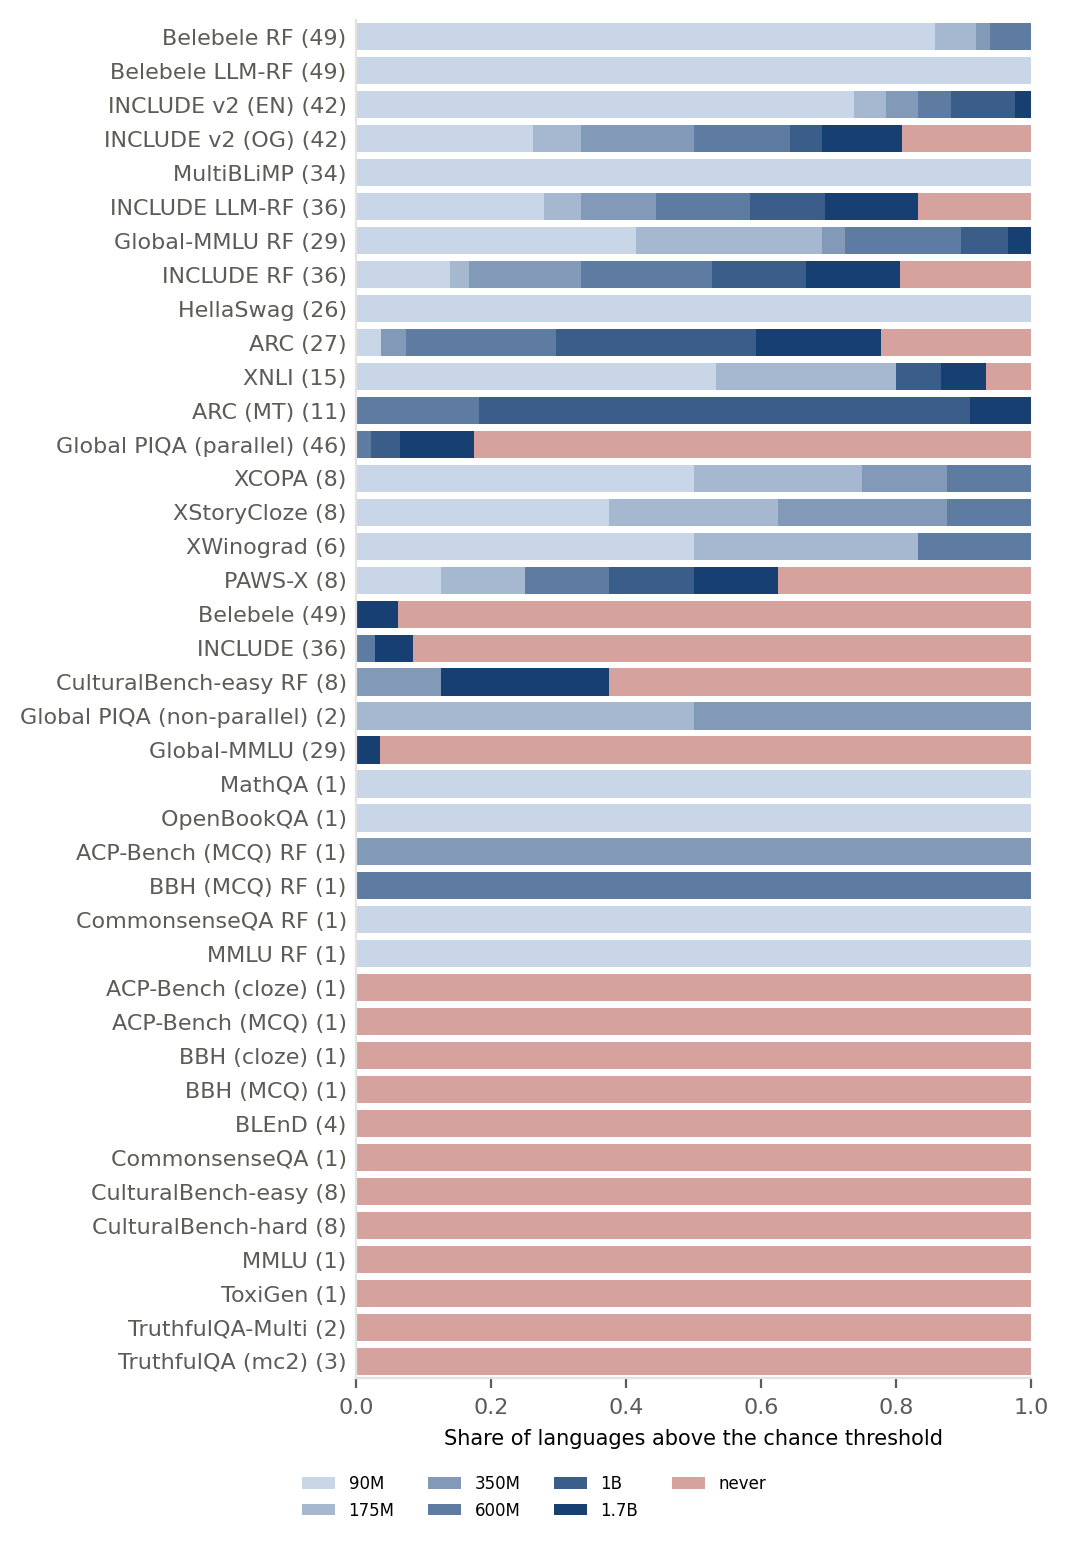
\includegraphics[width=0.48\textwidth]{figures/app_rq00_chance_share.png}
\hfill
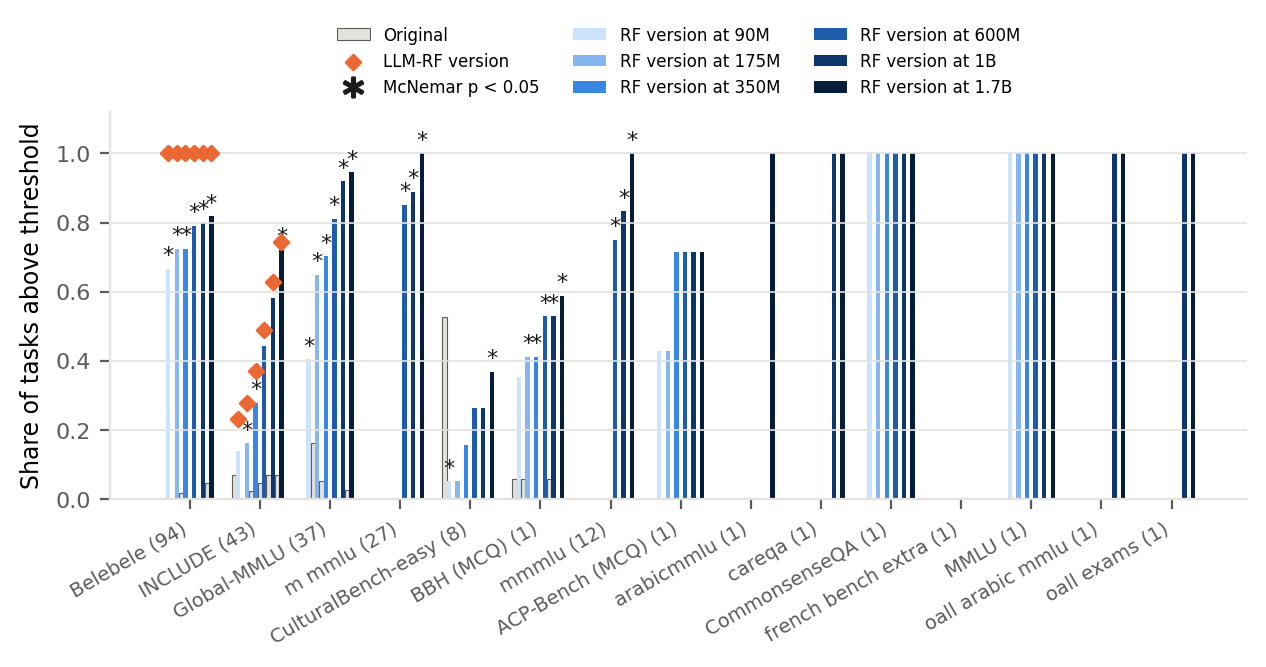
\includegraphics[width=0.48\textwidth]{figures/app_rq00_chance_reformulation.png}
\caption{\textbf{Left:} for each benchmark, the share of its trained languages that clear the above-chance gate, coloured by the smallest model size from which the score stays above chance at every larger size (red: never on this ladder). Benchmarks are ordered by the number of languages that pass at some size. \textbf{Right:} the letter-format families against their reformulated twins: the share of languages above the gate for the original (grey) and for the cloze twin at each size; diamonds mark the model-rewritten INCLUDE twin, and a star a McNemar exact test on the discordant languages with $p<0.05$.}
\label{fig:gate-share}
\end{figure}

Before asking whether a proxy reproduces the reference decision, we ask whether it measures anything at all.
Figure~\ref{fig:gate-share} (left) applies the gate of \S\ref{subsec:evaluation} to every benchmark--language task over the 50 languages of the largest mixture and reads, per task, the smallest size from which the score stays above chance.
Three groups emerge, and they follow the task format more than the capability the benchmark names.

\textbf{Measurable from the smallest proxy.}
Tasks that score a continuation or a minimal pair by likelihood clear chance at 175M in nearly every language: MultiBLiMP in all 34 languages, HellaSwag in 88\% of its 26, XCOPA in half of its languages at 175M and 88\% by 350M, XStoryCloze in 88\% by 350M, XWinograd in every language by 600M, and XNLI in 47\% at 175M and 93\% by 1.7B.
The cloze twins of the letter-format families behave the same way: Belebele-rf passes in 80\% of its 49 languages at 175M and in all of them by 1.7B, Global-MMLU-rf in 48\% at 175M and 97\% at 1.7B.
For these evaluations the smallest rung already carries a measurable signal, so the question of stage two, whether the signal ranks design variants like the reference, can be asked from 175M upwards.

\textbf{Measurable only from a larger size.}
A second group becomes measurable partway up the ladder.
ARC passes in 4\% of its 27 languages at 175M and in 52\% at 1.7B, with 37 of those points appearing at 1.7B alone; INCLUDE-rf rises gradually from 11\% at 175M to 81\% at 1.7B, PAWS-X from 12\% to 62\%, and the original Belebele clears chance in no language below 1B and in 18\% at 1.7B.
For these, a proxy below the size at which the task clears chance in a language reads noise for that language, whatever its decision accuracy would later be.

\textbf{Not measurable on this ladder.}
Global-MMLU in its original letter format is at chance in every one of its 29 languages at every size, as are CulturalBench-hard, the parallel Global PIQA cloze (45 of 46 languages), the original INCLUDE (32 of 36) and the English letter-format probes (MMLU, CommonsenseQA, BBH, ACP-Bench).
TruthfulQA moves in the opposite direction: the largest models are the furthest below chance.
Models of up to 1.7B non-embedding parameters trained on 100 tokens per parameter have not yet acquired what these evaluations ask for, or cannot express it in the letter-answer format, and any comparison of design variants on them at these sizes compares noise.

\textbf{The format hides part of the signal.}
Figure~\ref{fig:gate-share} (right) pairs each letter-format family with its cloze twin on the same languages and the same checkpoints.
Removing the answer letters lifts Belebele from 7\% to 62\% of its languages at 175M and from 10\% to 82\% at 1.7B, Global-MMLU from 0\% to 46\% and 95\%, and INCLUDE from 9\% to 72\% at 1.7B (77\% for the model-rewritten twin); McNemar's test on the discordant languages rejects chance at every size for Belebele and Global-MMLU.
The same items, scored as text, separate the ladder that the letter format reads as chance, so the exclusion rule of stage one is a property of the evaluation protocol as much as of the model.

\begin{figure}[t]
\centering
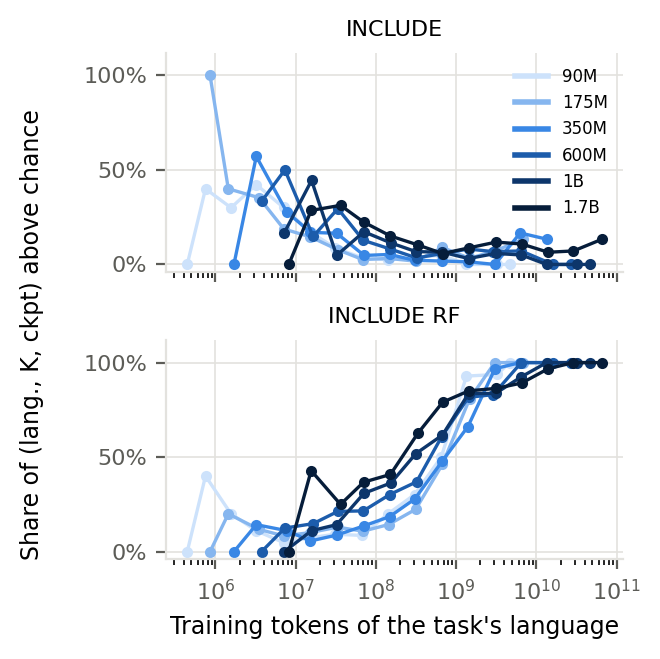
\includegraphics[width=0.45\textwidth]{figures/rq0.png}
\caption{The share of (language, mixture, checkpoint) cells above chance against the training tokens of the task's language that the checkpoint had seen, one line per model size, cells binned three per decade: INCLUDE in its original letter format (top) and as its cloze twin (bottom).}
\label{fig:gate-tokens}
\end{figure}

\textbf{Tokens of the language, not model size, set most thresholds.}
Figure~\ref{fig:gate-tokens} reads the same gate against the tokens of the task's language that a checkpoint had seen, pooling every mixture and every evaluated checkpoint of the seed-1904 runs.
The five size lines nearly coincide for most benchmarks: HellaSwag and XStoryCloze clear chance in half of their cells once the language has been seen for about $3\times10^{7}$ tokens, XNLI at $7\times10^{7}$, XWinograd at $3\times10^{8}$, INCLUDE-rf at $7\times10^{8}$, ARC at $1.5\times10^{10}$, and PAWS-X at $3\times10^{10}$, whatever the model size that saw them.
The two exceptions are the tasks that need capacity as well as exposure: on ARC and the original Belebele the 1.7B line leads the smaller sizes at equal tokens.
The practical output is a per-language exclusion rule: a language that a proxy has seen for fewer tokens than the benchmark's threshold should not enter a decision on that benchmark, at any model size, because its score adds variance to any aggregate without adding information.
% Anomalies to resolve before this section is final:
% - cultural_bench_easy (original) passes in 84% of languages at 175M and in 0-11% above it: the 175M runs score 0.45-0.65 from the first checkpoint, English-only cells included, on 7-59 items per country. An answer-key or length bias the smallest models exploit, not a skill; its rf twin (5% -> 37%) is the honest reading. Excluded from the text above.
% - rfgm_belebele is absent from the gate: the ladder report the gate read (2026-09-25 15:18) has no rfgm_belebele columns, while the later rq01 tokens-seen table has them at 99.8% above chance from the first checkpoint, which itself needs a look (a rewrite that is above chance at 10^6 tokens is suspicious).
% - toxigen (1 language) passes at 175M only; truthfulqa declines with size.
